\maketitle
\chapter{I risultati e il report}

Si proverà adesso a filtrare un’immagine 32x32 pixel utilizzando in un primo caso un filtro Gaussiano 3x3 con fattore di normalizzazione pari a sedici e, in un secondo caso, un filtro di Sobel verticale 3x3 con fattore di normalizzazione pari a quattro. 

In ambo i casi verranno poi valutati i corrispettivi report. Per effettuare la simulazione è stato impiegato un codice Matlab che, con una generica immagine in ingresso, dà in uscita la stessa immagine  in scala di grigi ridimensionata ad un formato 32x32 pixel.

 Successivamente da questa immagine vengono poi estratte i valori dei pixel e trasformati in due file testuali: uno organizzato in una struttura vettoriale 1024x1 da usare per il testbench del circuito e uno composto da una struttura matriciale 32x32 che sarà impiegato per la valutazione del confronto dei valori ottenuti con il circuito attraverso un file Excel. 

Dopo aver effettuato i testbench per i due filtri scelti, viene utilizzato l'Excel che, presi i valori dei pixel in formato 32x32 in ingresso, effettua l’operazione di filtraggio specificatamente per i coefficienti e il divisore del filtro impostato restituendoci, di fatto, i pixel correttamente filtrati. 

Una panoramica generale del seguente foglio Excel è la seguente:
\begin{figure}[H]  
	\hspace{-3.5 cm}
	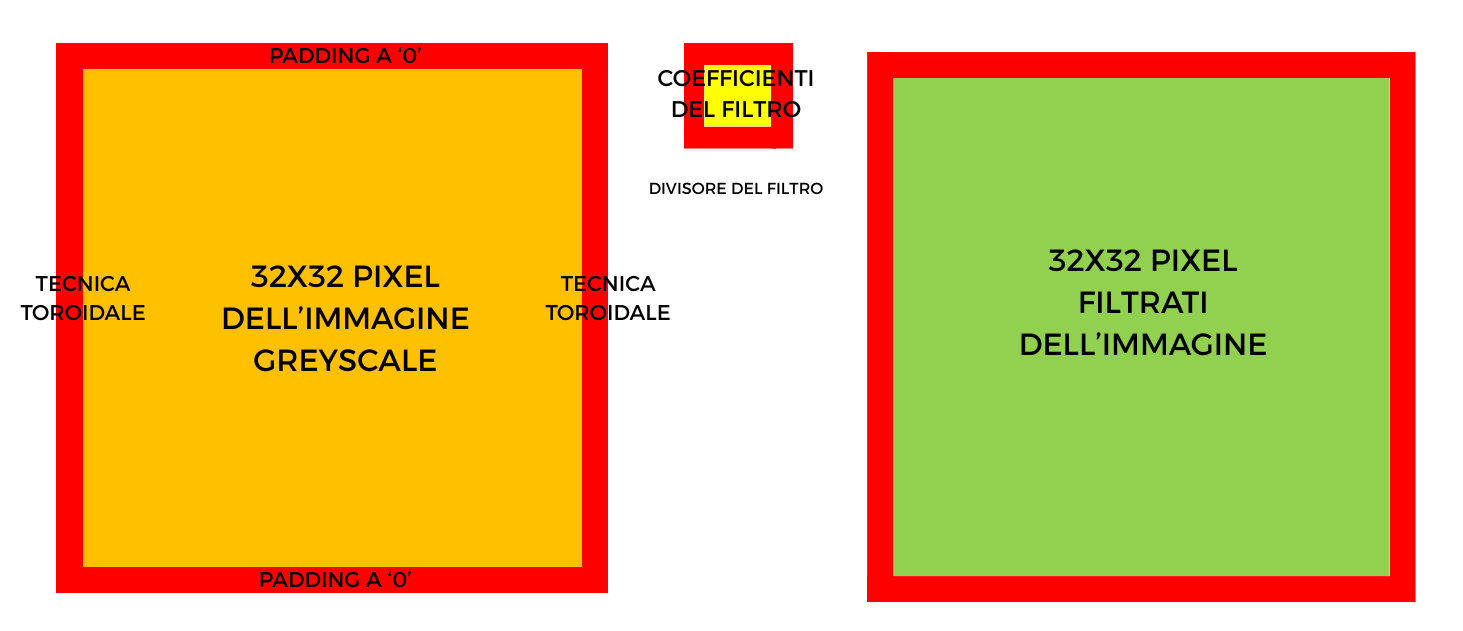
\includegraphics[width=1.5\textwidth]{file_relazione/imgs/excel.png}
\end{figure}

Avendo quindi a disposizione in modo preventivo i valori dei pixel originali e filtrati, è stato possibile confrontare tramite il file Excel l’immagine filtrata in uscita dal circuito con quella attesa, constatando il corretto filtraggio in entrambi i casi. 

L'immagine originale analizzata è stata creata con un semplice script MATLAB ed è la seguente:
\begin{figure}[H]  
	\centering
	
\includegraphics[width=0.7\textwidth]{file_relazione/imgs/scacchiera.png}
\end{figure}

\section{Il filtro Gaussiano}
Prendendo in considerazione il filtro Gaussiano, esso sarà composto dai seguenti coefficienti:
\begin{table}[H]
\begin{tabular}{|c|c|c|}
\hline
1 & 2 & 1 \\ \hline
2 & 4 & 2 \\ \hline
1 & 2 & 1 \\ \hline
\end{tabular}
\end{table}

Andando ad impostare i seguenti parametri nel progetto, verrà successivamente avviata la simulazione post implementazione ad una temperatura di 25°C. Normalizzando ogni pixel filtrato per un fattore pari a sedici, l’immagine filtrata ottenuta sarà la seguente:
\begin{figure}[H]  
	\centering
	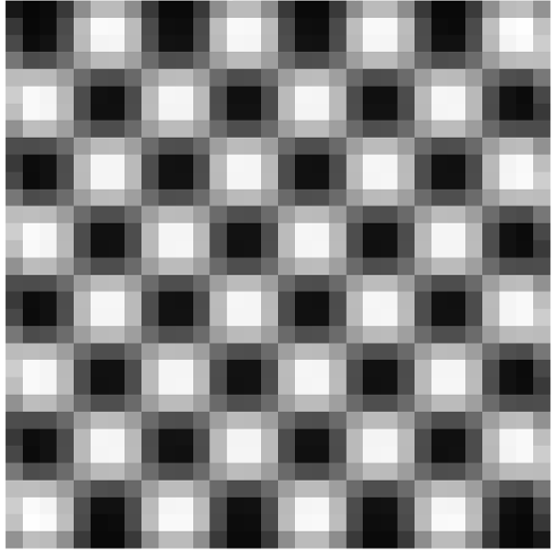
\includegraphics[width=0.7\textwidth]{file_relazione/imgs/scacchiera_filtrata.png}
\end{figure}

Generando i report relativi all’utilizzo di risorse, all’uso di potenza e al timing si otterranno i seguenti risultati:
\begin{figure}[H]  
	\hspace{-2 cm}
	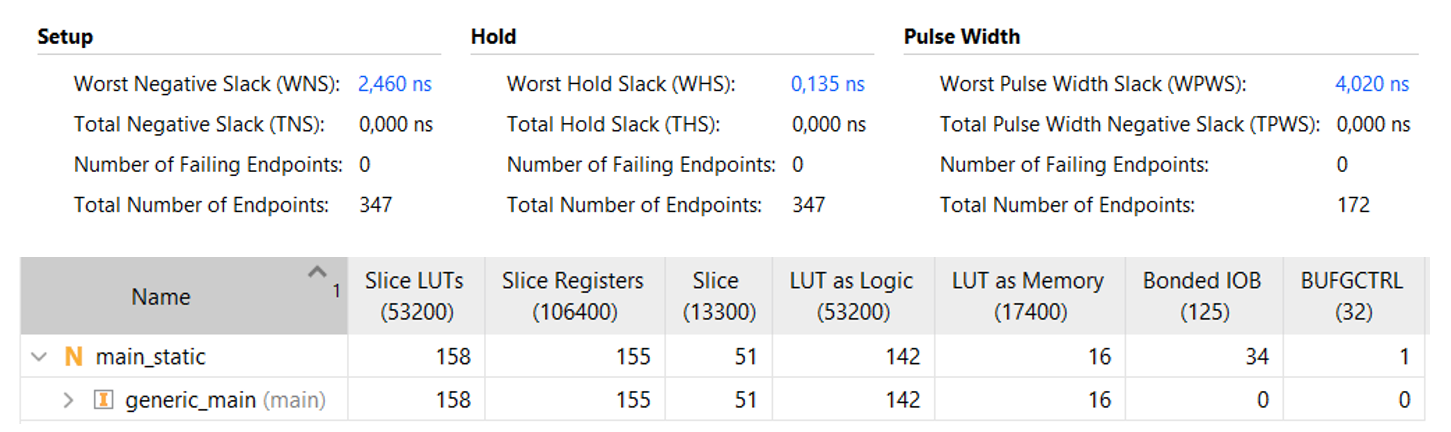
\includegraphics[width=1.3\textwidth]{file_relazione/imgs/report1.png}
\end{figure}
\begin{figure}[H]  
	\hspace{-2 cm}
	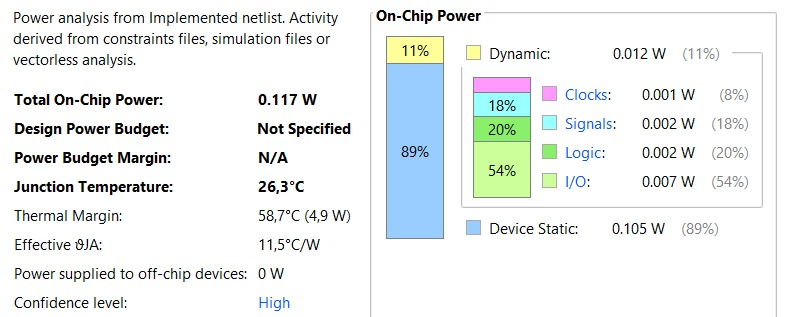
\includegraphics[width=1.3\textwidth]{file_relazione/imgs/report2.jpeg}
\end{figure}

\section{Il filtro di Sobel (verticale)}
Prendendo in considerazione il filtro di Sobel verticale, esso sarà composto dai seguenti coefficienti:
\begin{table}[H]
\begin{tabular}{|c|c|c|}
\hline
-1 & 0 & 1 \\ \hline
-2 & 0 & 2 \\ \hline
-1 & 0 & 1 \\ \hline
\end{tabular}
\end{table}

Andando ad impostare i seguenti parametri nel progetto, verrà successivamente avviata la simulazione post implementazione ad una temperatura di 25°C. 
Normalizzando ogni pixel filtrato per un fattore pari a quattro, l’immagine filtrata ottenuta sarà la seguente:
\begin{figure}[H]  
	\centering
	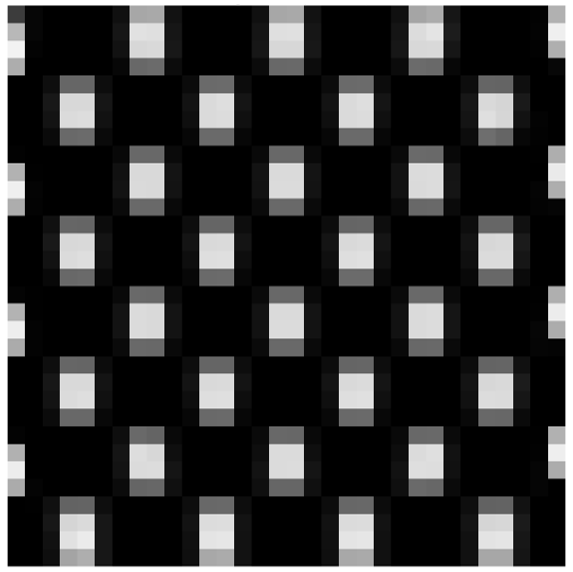
\includegraphics[width=0.7\textwidth]{file_relazione/imgs/scacchiera_sobel.png}
\end{figure}

Generando i report relativi all’utilizzo di risorse, all’uso di potenza e al timing si otterranno i seguenti risultati:
\begin{figure}[H]  
	\hspace{-2 cm}
	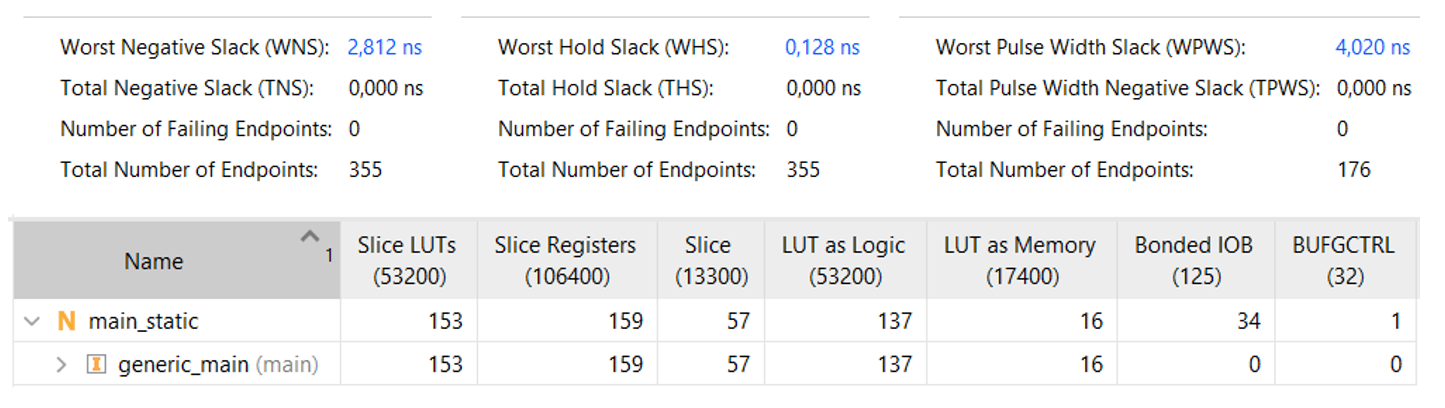
\includegraphics[width=1.3\textwidth]{file_relazione/imgs/report3.png}
\end{figure}
\begin{figure}[H]  
	\hspace{-2 cm}
	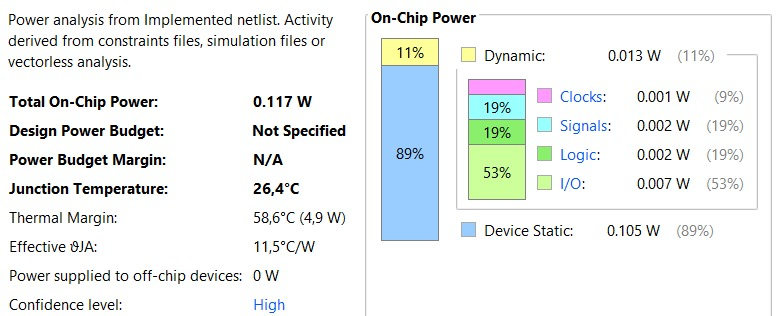
\includegraphics[width=1.3\textwidth]{file_relazione/imgs/report4.jpeg}
\end{figure}
Dopo aver implementato i due filtri, è possibile notare delle differenze tra i report. La prima risiede in un WNS più alto per il circuito col filtro di Sobel verticale. Si passa infatti da un WNS di 2,46 ns ad un WNS di 2,812ns e quindi 0,352ns in più. Ipotizzando di ridurre fino a zero il WNS in entrambi i casi (idealità), tale operazione permetterebbe al circuito col filtro di Sobel di lavorare ad una frequenza massima teorica maggiore del 4,89\% rispetto al caso con il filtro Gaussiano. Questo risultato è dovuto al fatto che col filtro di Sobel non viene utilizzata la colonna centrale del kernel, e i risultati calcolati saranno più piccoli in modulo con una propagazione dei riporti più contenuta. Calcolare prodotti per zero è infatti meno dispendioso in termini computazionali, potendo anche fisicamente eliminare le linee per i coefficienti nulli. Grazie a questo funzionamento alleggerito, il risultato in uscita vedrà un path critico più corto che gli permetterà di attraversare la logica più velocemente. Per questi motivi, si vedrà una riduzione delle LUT utilizzate e, a fronte di una potenza dinamica maggiore di 1mW, la quota di potenza relativa alla logica scenderà dal 20\% al 19\% mentre quella relativa agli I/O dal 54\% al 53\%. Questo conferma che la parte di calcolo è effettivamente più efficiente nel Sobel.

